% !TeX spellcheck = it_IT
\newpage
\section{Design pattern}
La progettazione non è solo un processo creativo. Il progettista può infatti seguire una serie di regole pratiche, appunto i design patterns, che descrivono il cuore della soluzione ad un problema frequente in modo che questa possa essere riutilizzata tante volte.\\

Nel software in particolare i pattern (soluzioni create in passato) vengono utilizzati per avere una maggiore \textbf{produttività} e rendere i progetti più \textbf{flessibili}.\\

\subsection{Gang of Four}
\subsubsection{Classificazione}
Nell'ambito della \textbf{progettazione di dettaglio}, \textbf{GoF} i pattern sono classificati in base al loro scopo e divisi in tre categorie:
\begin{itemize}
	\item \textbf{Creazionali}: riguardano la creazione di oggetti
	\begin{itemize}
		\item \textit{Abstract Factory}
		\item \textit{Builder}
		\item \textit{Factory Method}
		\item \textit{Prototype}
		\item \textit{Singleton}
	\end{itemize}
	\item \textbf{Strutturali}: riguardano la composizione di classi ed oggetti
	\begin{itemize}
		\item \textit{Adapter}
		\item \textit{Bridge}
		\item \textit{Composite}
		\item \textit{Decorator}
		\item \textit{Façade}
		\item \textit{Flyweight}
		\item \textit{Proxy}
	\end{itemize}
	\item \textbf{Comportamentali}: riguardano le interazioni tra classi ed oggetti e la suddivisione delle loro responsabilità
	\begin{itemize}
		\item \textit{Chain of responsibility}
		\item \textit{Command}
		\item \textit{Interpreter}
		\item \textit{Iterator}
		\item \textit{Mediator}
		\item \textit{Memento}
		\item \textit{Observer}
		\item \textit{State}
		\item \textit{Strategy}
		\item \textit{Template}
		\item \textit{Visitor}
	\end{itemize}
\end{itemize}

\newpage
\subsubsection{Template}
Un buon template per un pattern secondo GoF è il seguente:
\begin{table}[!h]
	\centering
	\begin{tabular}{|c|c|}
		\hline
		\textbf{Pattern name and classification} & Un nome breve e conciso per un pattern ed il suo tipo \\
		\hline
		\textbf{Intent} & Una breve frase su cosa fa il pattern \\
		\hline
		\textbf{Also known as} & Altri nomi \\
		\hline
		\textbf{Motivation} & Uno scenario che mostri perché è utile \\
		\hline
		\textbf{Applicability} & Situazioni dove può essere usato \\
		\hline
		\textbf{Structure} & Rappresentazione grafica \\
		\hline
		\textbf{Participants} & Le classi e gli oggetti che lo compongono\\
		\hline
		\textbf{Collaborations} & Come i partecipanti rispettano le loro responsabilità \\
		\hline
		\textbf{Consequences} & Pro e contro \\
		\hline
		\textbf{Implementation} & Suggerimenti e tecniche per l'implementazione \\
		\hline
		\textbf{Sample code} & Frammenti di codice per una semplice implementazione \\
		\hline
		\textbf{Known users} & Esempi in sistemi reali \\
		\hline
		\textbf{Related patterns} & Altri pattern strettamente correlati \\
		\hline
	\end{tabular}
\end{table}

\subsubsection{Notazione}
GoF utilizza come notazione la \textbf{Object Modeling Technique}.
\begin{center}
	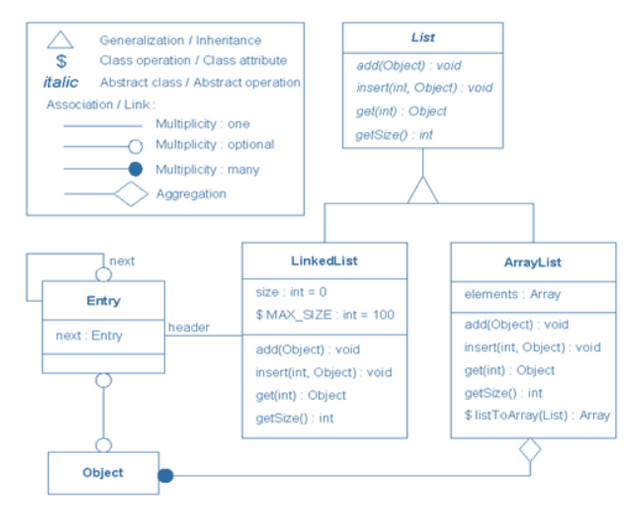
\includegraphics[scale=.5]{gof}
\end{center}

\subsection{Strategy}
\subsection{State}